%% -*- TeX-engine: luatex; ispell-language: "russian" -*-

\documentclass[a4paper,12pt]{article}
\usepackage{subcaption}
\input{handout-base}

\newcounter{mypar}
\newcommand{\mypar}{\stepcounter{mypar}\paragraph{\arabic{mypar}.}}

\begin{document}
\subsection*{Домашнее задание №9: <<Каракули и нейросети>>}

\begin{tabular}{@{}lr}
  \textbf{Дедлайн 1} (20 баллов): & 14 мая, 23:59 \\
  \textbf{Дедлайн 2} (10 баллов): & 21 мая, 23:59
\end{tabular}

Домашнее задание нужно написать на Python и сдать в виде одного файла.
Правило именования файла: \texttt{name\_surname\_9.py}. Например, если
вас зовут Иван Петров, то имя файла должно быть: \texttt{ivan\_petrov\_9.py}.

\makebox[\linewidth]{\hrulefill}

\begin{figure}[h!]
  \centering
  
\includegraphics[width=.7\linewidth]{images/images}
\end{figure}


В этом домашнем задании мы продолжим тему распознавания образов. Для тестирования нашего алгоритма будем использовать датасет MNIST \footnote{\url{http://en.wikipedia.org/wiki/MNIST_database}}. 

MNIST (Mixed National Institute of Standards and Technology database) является основной базой при тестировании систем распознавания образов, а также широко используемой для обучения и тестирования алгоритмов машинного обучения. Она была создана перегруппировкой образов из оригинальной базы NIST, которая являлась достаточно сложной для распознавания. Кроме этого, были выполнены определенные преобразования (образы были нормализованы и сглажены для получения градаций серого цвета). 

\mypar Реализуйте обучение нейронной сети с помощью метода обратного распространения ошибки (Back Propagation). 


В качестве функции активации рекомендуется использовать сигмоиду.

\clearpage
Структура класса приведена ниже:
\begin{python3}	
class NeuralNetwork:
    def __init__(self, layers):
        self.num_layers = len(layers)
        self.layers = layers
        ...

    def train(self, X, y, n_iter=100, learning_rate=1): 
        ...
        
    def feedforward(self, X): 
        ...
        
    def backpropagation(self, X, y):
        ...
    	
    def predict(self, X):
        ...

\end{python3}
При реализации метода \pythoninline{train} может быть полезно обратиться к своей реализации метода стохастического градиента из предыдущих домашних заданий.

\mypar Дополните реализацию методом \pythoninline{predict}, который прогоняет все объекты из переданной матрицы \pythoninline{X} через полученную нейросеть. Предполагается, что метод возвращает индекс нейрона, на котором значение на выходном слое максимально.


\mypar Так как на этот раз мы используем стандартный датасет, в \pythoninline{scikit-learn} есть функция, позволяющая его легко получить:

\begin{python3}
from sklearn import datasets
from sklearn.cross_validation import train_test_split
dataset = datasets.fetch_mldata("MNIST Original")
trainX, testX, trainY, testY = train_test_split(
    dataset.data / 255.0, dataset.target.astype("int0"), test_size = 0.3)
\end{python3}

\mypar Для визуализации датасета можно воспользоваться функцией \pythoninline{visualize_mnist} из файла по ссылке. \footnote{\url{https://gist.github.com/ktisha/95fcee0ed79236c7e6e5}} 

Картинка должна выглядеть подобным образом:

\begin{figure}[h!]
  \centering
  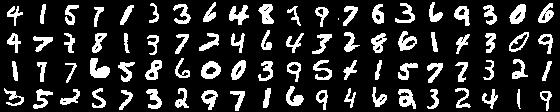
\includegraphics[width=.7\linewidth]{images/mnist}
\end{figure}

\mypar Пример использования полученной сети:
\begin{python3}
nn = NeuralNetwork([train_X.shape[1], 10])
nn.train(trainX, trainY)
nn.predict(testY)
\end{python3}
Обратите внимание, что на первом слое нам нужно число нейронов, равное количеству признаков (в данном случае, количеству пикселей), а на выходном слое количество нейронов, равное количеству классов объектов (в нашем случае это цифры 0-9).

\mypar Оценивать качество классификации в этот раз мы будем простым подсчетом отношения правильно классифицированных объектов к общему количеству объектов в выборке.

\mypar Ответьте на вопрос: как меняется качество классификации при изменении количества слоев сети и количества нейронов на каждом слое?
 
\end{document}
